\documentclass[man,a4paper,12pt,floatsintext,nolmodern,notab]{apa7}
\usepackage[american]{babel}
\usepackage{fontspec}
\setmainfont{TeX Gyre Termes}
\setsansfont{TeX Gyre Heros}
\newfontfamily\cjkfont{HaranoAjiMincho-Regular.otf}
\usepackage{graphicx}
\usepackage{booktabs}
\usepackage{array}
\usepackage{xurl}
\urlstyle{same}
\hypersetup{hidelinks}
\usepackage{longtable}
\usepackage{needspace}
\usepackage{setspace}
\usepackage{microtype}
\newcommand{\tablefont}{\small}

\title{Effects of Concrete and Virtual Manipulatives on Mathematics Learning in Primary and Lower Secondary Students: A Meta-Analysis}
\shorttitle{EFFECTS OF CONCRETE AND VIRTUAL MANIPULATIVES}
\authorsnames{Society for Educational Data Analysis (SEDA)}
\authorsaffiliations{Generative AI paper}
\abstract{Manipulatives are objects and digital tools that students handle to represent mathematical ideas, and teachers need to know whether using them is linked to higher achievement. Using an automated workflow in which every extracted number was verified against the full text, 8 open-access studies (\textit{N} = 499) were pooled with a random-effects model. The pooled effect was \textit{g} = 1.49, 95\% CI [0.97, 2.02], with \textit{I}² = 81.1\%. In these eight small studies, instruction with manipulatives was associated with higher post-test scores, but the effects varied widely, so the evidence is preliminary.}
\keywords{meta-analysis, manipulatives, mathematics achievement, virtual manipulatives, primary education, lower secondary education}
\authornote{This is a “Generative AI paper” produced automatically by the Society for Educational Data Analysis (SEDA) with generative AI. Large language models (gemma4:12b (Ollama; drafts) and claude-sonnet-5-5 (Claude Code; review and revision)) were used to screen records, extract data, and draft the Introduction, Discussion, and Conclusion; all statistics were computed by software. The paper has not been peer reviewed.

The Japanese version of this paper, with identical content, is available at \url{https://raw.githubusercontent.com/k518-2026/MetaAnalysisToWP/main/reports/2026-10-11-math-manipulatives/paper-ja.pdf}. Published October 11, 2026.

Data and code are available at \url{https://github.com/k518-2026/MetaAnalysisToWP}. © 2026 Society for Educational Data Analysis (SEDA).}
\begin{document}
\maketitle
Mathematics in primary and lower secondary school moves from concrete quantities to symbolic notation, and many students find the abstract ideas hard to grasp. Teachers therefore often look for ways to make mathematical ideas visible and easy to act on.

Manipulatives are objects or digital tools that students handle or move to represent mathematical ideas. Concrete manipulatives include plastic cubes and fraction tiles (Liggett, 2017; Magto \& Salazar, 2025), whereas virtual manipulatives are interactive digital tools, such as applets for geometry and algebra (Ejiofor-Chima, 2025; Mahmuti \& Arifi, 2025; Temür \& Sevimli, 2024). The included studies examined them in topics such as fractions (Magto \& Salazar, 2025; Ukdem \& Çeti̇n, 2022), geometry (Carcueva et al., 2025; Ejiofor-Chima, 2025; Mahmuti \& Arifi, 2025; Scippo et al., 2025) and algebra (Temür \& Sevimli, 2024).

Each study involves a small number of classes and a particular topic, so a single study gives only a limited picture. A quantitative synthesis can put the results on the same scale, estimate the typical size of the difference between groups, show how much the results differ across studies, and ask whether the difference looks different in primary and lower secondary school.

The purpose of this meta-analysis was to estimate the overall difference in mathematics achievement between students taught with concrete or virtual manipulatives and students taught without them in grades 1 to 9. Our research question was: how large is the difference in post-test mathematics achievement between instruction with manipulatives and instruction without them, and does it differ between school levels?

\section{Method}
\subsection{Literature Search}
Searches were run on October 11, 2026 in two open bibliographic sources. OpenAlex was searched in the title and abstract fields with the query “(manipulatives OR “concrete materials” OR “virtual manipulatives” OR “hands-on”) AND (mathematics OR math OR arithmetic OR geometry) AND (elementary OR primary OR “middle school” OR “junior high” OR “lower secondary” OR grade OR children OR pupils)”, restricted to open-access journal articles published in 2012 or later and classified in the Education or Developmental and Educational Psychology subfields. J-STAGE, the Japanese journal platform, was searched in the abstract field with the keywords “{\cjkfont 具体物} {\cjkfont 算数}”, “{\cjkfont 操作活動} {\cjkfont 算数} {\cjkfont 効果}” (2012 or later) to include studies published in Japan.

\subsection{Eligibility Criteria}
Studies were eligible if they (a) sampled students in grades 1-9 (primary/elementary school and lower secondary/middle/junior high school, ages about 6-15); Exclude preschool-only, upper secondary-only, university, adult, and teacher/pre-service teacher samples; (b) examined instruction using concrete or virtual manipulatives; (c) compared it with instruction without manipulatives (e.g., symbolic or textbook-only instruction); (d) measured a mathematics achievement test; and (e) reported statistics sufficient to compute a standardized mean difference. Reviews, qualitative studies, single-case designs, and single-group pre-post designs were excluded.

\subsection{Screening and Data Extraction}
Screening and data extraction used language models (gemma4:12b (Ollama; drafts) and claude-sonnet-5-5 (Claude Code; review and revision)). The first model (Ollama) rated each title and abstract against the eligibility criteria; this screening was not reviewed. Full texts (PDF) of the highest-rated records were retrieved and converted to plain text, and the same model drafted the study characteristics and summary statistics. A second model (Claude Code) then checked each draft against the full text, corrected it, and judged eligibility. Every extracted number was then checked by software against the full text, and a study was excluded from the synthesis if any extracted number could not be found verbatim. The model also classified the comparison condition of each study as passive (no intervention, a waitlist, or regular lessons) or active (an alternative intervention aimed at the same outcome) and quoted the passage supporting the classification; a classification whose quotation could not be found in the full text was recorded as unclear. No human reviewer verified the screening or the extraction. When more than 10 studies qualified, the 10 with the highest screening ratings were retained.

\subsection{Effect Sizes}
Standardized mean differences were computed as Hedges’ g (Hedges, 1981) from post-test means, standard deviations, and group sizes; when these were unavailable, from independent-samples t statistics, from F statistics with one numerator degree of freedom, or from reported d or g values. Positive values indicate higher scores in the intervention group. One effect size per study was used.

\subsection{Statistical Analysis}
Effect sizes were pooled with a random-effects model in which the between-study variance (\textit{τ}²) was estimated with the DerSimonian–Laird method (DerSimonian \& Laird, 1986). Confidence intervals and tests of the pooled effect used the Hartung–Knapp–Sidik–Jonkman (HKSJ) adjustment, which is recommended when the number of studies is small (Hartung \& Knapp, 2001; IntHout et al., 2014). Heterogeneity was assessed with Q, \textit{I}² (Higgins \& Thompson, 2002), \textit{τ}², and a 95\% prediction interval. Subgroup analyses by school level (elementary: grades 1–6; lower secondary: grades 7–9) were conducted when each level included at least two studies. A further subgroup analysis compared studies with a passive comparison condition with those with an active comparison condition, again requiring at least two studies per type; studies whose comparison type was unclear were left out of this comparison only. Robustness was examined with leave-one-out analysis, and Egger’s regression test (Egger et al., 1997) was planned only when at least 10 studies were available. Effect magnitudes were interpreted with conventional benchmarks (Cohen, 1988). Analyses followed standard formulas (Borenstein et al., 2009) implemented in open-source JavaScript code (\url{https://github.com/k518-2026/MetaAnalysisToWP}).

\section{Results}
\subsection{Study Selection}
The searches returned 200 records from OpenAlex (of 1009 matching the query) and 11 from J-STAGE, for 206 unique records. Of the 200 records with abstracts that were screened, 27 were rated as potentially eligible. Full texts of 27 records were examined: 12 could not be retrieved or read, 6 did not meet the eligibility criteria, 0 did not report sufficient statistics, 0 contained extracted numbers that could not be verified in the text, and 1 yielded implausible values. In total, 8 studies were included in the meta-analysis.

\subsection{Study Characteristics}
Table 1 summarizes the country, grade, design, sample size, and effect size of each included study (Carcueva et al., 2025; Ejiofor-Chima, 2025; Liggett, 2017; Magto \& Salazar, 2025; Mahmuti \& Arifi, 2025; Scippo et al., 2025; Temür \& Sevimli, 2024; Ukdem \& Çeti̇n, 2022). The studies comprised 499 participants in total and were conducted in Turkey, Italy, Kosovo, Canada, Philippines, Nigeria. By school level, 3 studies sampled elementary (grades 1–6) students, 5 studies sampled lower secondary (grades 7–9) students. Sample sizes ranged from 32 to 120, and individual effect sizes ranged from \textit{g} = 0.68 to \textit{g} = 2.33.

\par\vspace{4pt}
{\tablefont\singlespacing\setlength{\LTpre}{6pt}\setlength{\LTpost}{2pt}
\begin{longtable}{>{\raggedright\arraybackslash}p{0.2600\dimexpr\linewidth-12\tabcolsep\relax}>{\raggedright\arraybackslash}p{0.1100\dimexpr\linewidth-12\tabcolsep\relax}>{\raggedright\arraybackslash}p{0.1200\dimexpr\linewidth-12\tabcolsep\relax}>{\raggedright\arraybackslash}p{0.2300\dimexpr\linewidth-12\tabcolsep\relax}>{\raggedright\arraybackslash}p{0.0700\dimexpr\linewidth-12\tabcolsep\relax}>{\raggedright\arraybackslash}p{0.2100\dimexpr\linewidth-12\tabcolsep\relax}}
\multicolumn{6}{@{}l@{}}{\textbf{Table 1}} \\
\multicolumn{6}{@{}p{\linewidth}@{}}{\textit{Overview of the Included Studies}} \\[3pt]
\toprule
Study & Country & Grade & Design & \textit{N} & \textit{g} [95\% CI] \\
\midrule
\endfirsthead
\toprule
Study & Country & Grade & Design & \textit{N} & \textit{g} [95\% CI] \\
\midrule
\endhead
Ukdem and Çeti̇n (2022) & Turkey & Grade 3 & quasi-experimental (two experimental groups and one control group) & 41 & 1.42 [0.74, 2.09] \\
Scippo et al. (2025) & Italy & Grade 4 & quasi-experimental & 35 & 0.68 [0.02, 1.35] \\
Mahmuti and Arifi (2025) & Kosovo & Grade 7 & quasi-experimental & 32 & 1.05 [0.33, 1.77] \\
Liggett (2017) & Canada & Grade 2 & randomized controlled trial & 43 & 1.59 [0.92, 2.27] \\
Temür and Sevimli (2024) & Turkey & Grade 7 & quasi-experimental & 60 & 1.61 [1.04, 2.19] \\
Magto and Salazar (2025) & Philippines & Grade 7 & quasi-experimental & 84 & 0.83 [0.38, 1.27] \\
Ejiofor-Chima (2025) & Nigeria & Grade 9 (JSS3) & quasi-experimental & 120 & 2.33 [1.87, 2.80] \\
Carcueva et al. (2025) & Philippines & Grade 7 & quasi-experimental & 84 & 2.31 [1.76, 2.86] \\
\bottomrule
\end{longtable}
\noindent \textit{Note.} CI = confidence interval. \textit{g} = Hedges’ g (positive values favor the intervention). Grades and designs were extracted automatically from the full texts.\par}
\vspace{6pt}
Table 2 lists the intervention, comparison condition, and outcome measure of each study. All 8 studies compared an intervention group with a comparison group on a post-test.

\par\vspace{4pt}
{\tablefont\singlespacing\setlength{\LTpre}{6pt}\setlength{\LTpost}{2pt}
\begin{longtable}{>{\raggedright\arraybackslash}p{0.2000\dimexpr\linewidth-8\tabcolsep\relax}>{\raggedright\arraybackslash}p{0.3200\dimexpr\linewidth-8\tabcolsep\relax}>{\raggedright\arraybackslash}p{0.2400\dimexpr\linewidth-8\tabcolsep\relax}>{\raggedright\arraybackslash}p{0.2400\dimexpr\linewidth-8\tabcolsep\relax}}
\multicolumn{4}{@{}l@{}}{\textbf{Table 2}} \\
\multicolumn{4}{@{}p{\linewidth}@{}}{\textit{Interventions, Comparison Conditions, and Outcome Measures}} \\[3pt]
\toprule
Study & Intervention & Comparison & Outcome \\
\midrule
\endfirsthead
\toprule
Study & Intervention & Comparison & Outcome \\
\midrule
\endhead
Ukdem and Çeti̇n (2022) & concrete manipulative-assisted fraction instruction (Experiment 1) & traditional teaching in the mathematics curriculum [passive] & Fraction Comprehension Test (post-test) \\
Scippo et al. (2025) & tessellation program with GeoGebra and 3D-printed materials & standard geometry curriculum (plane figures and angles) [passive] & geometry learning test (post-test) \\
Mahmuti and Arifi (2025) & instruction with virtual manipulatives & traditional methods [passive] & post-test scores on perimeter and area \\
Liggett (2017) & instruction using plastic unifix cubes & instruction without manipulatives [passive] & math achievement test scores \\
Temür and Sevimli (2024) & activity-based teaching enriched with virtual manipulatives & activities in the current secondary school mathematics textbook [passive] & Algebra Misconception Identification Test \\
Magto and Salazar (2025) & instruction using tangible mathematics manipulatives (fraction circles, bars, tiles, and operational tiles) & control group (instruction not described) & mathematics achievement test (rational number operations) \\
Ejiofor-Chima (2025) & instruction using virtual manipulatives (Right Triangle Solver and Pythagorean theory applets) & lecture-based instruction [passive] & Geometry Achievement Test (GAT) \\
Carcueva et al. (2025) & manipulative-based instruction & traditional teaching [passive] & 40-item Achievement Test \\
\bottomrule
\end{longtable}
\noindent \textit{Note.} Extracted and summarized automatically from the full texts. [passive] = no intervention or regular lessons; [active] = an alternative intervention aimed at the same outcome. Unclear cases carry no label.\par}
\vspace{6pt}
\subsection{Overall Effect}
Figure 1 shows the forest plot. Each square marks the effect size of one study, with its size proportional to the study’s weight, and each horizontal line marks the 95\% confidence interval; the diamond at the bottom is the pooled estimate. 8 of the 8 studies had positive effect sizes, and the confidence intervals of 8 studies did not include zero. The study with the largest weight was Magto and Salazar (2025) (13.7\%).

\begin{figure}[!htbp]
\caption{Forest Plot of Individual and Pooled Effect Sizes}
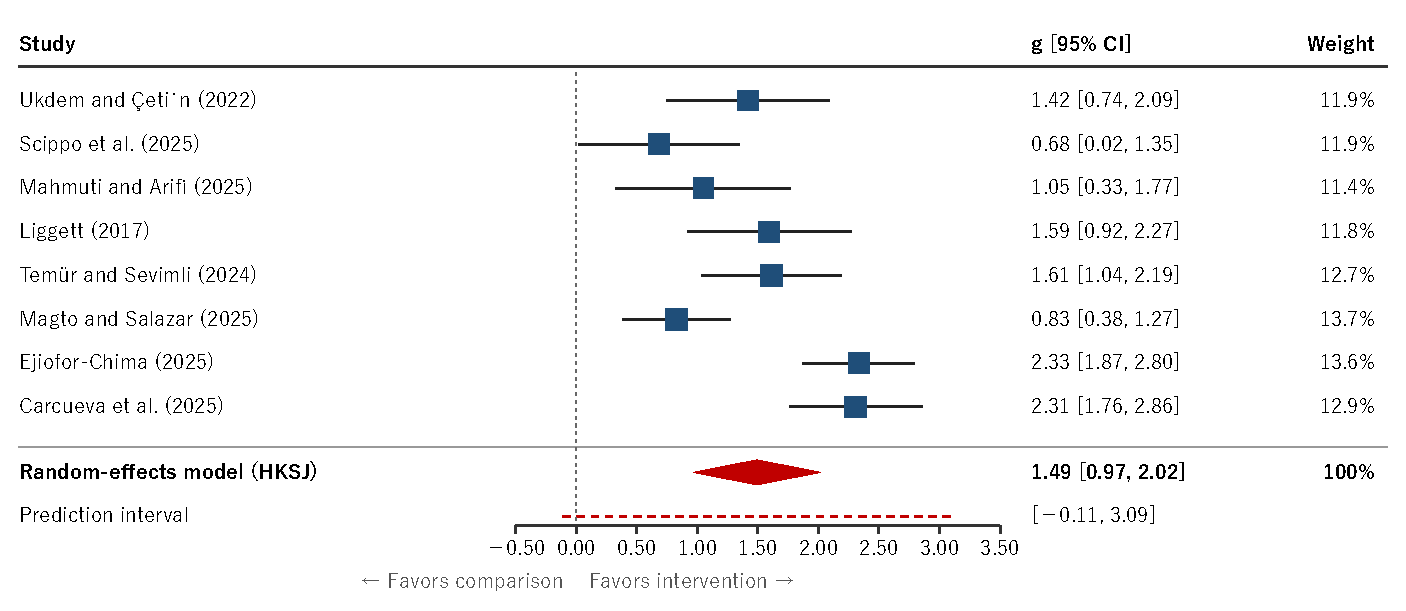
\includegraphics[width=\linewidth]{forest-en.pdf}
\figurenote{Squares show study effect sizes (size proportional to weight), lines show 95\% confidence intervals, the diamond shows the pooled estimate, and the dashed line shows the prediction interval.}
\end{figure}
The random-effects model yielded a pooled effect of \textit{g} = 1.49, 95\% CI [0.97, 2.02], \textit{t}(7) = 6.70, p < .001, which corresponds to a large effect by conventional benchmarks. The fixed-effect estimate was \textit{g} = 1.53. Table 3 summarizes these estimates.

\subsection{Heterogeneity}
Heterogeneity was considerable, \textit{Q}(7) = 37.04, p < .001, \textit{I}² = 81.1\%, \textit{τ}² = 0.370. The 95\% prediction interval ranged from \ensuremath{-}0.11 to 3.09.

\subsection{Subgroup and Sensitivity Analyses}
For elementary (grades 1–6) samples, \textit{g} = 1.23, 95\% CI [0.03, 2.43] (\textit{k} = 3); for lower secondary (grades 7–9) samples, \textit{g} = 1.64, 95\% CI [0.77, 2.51] (\textit{k} = 5). The difference between school levels was not statistically significant, \textit{Q}(1) = 0.94, \textit{p} = .333. A subgroup analysis by type of comparison condition (passive versus active) was not conducted because fewer than two studies were available for at least one type. Leave-one-out estimates ranged from 1.36 to 1.60. Publication bias was not tested because fewer than 10 studies were included. The subgroup estimates are also shown in Table 3.

\par\vspace{4pt}
{\tablefont\singlespacing\setlength{\LTpre}{6pt}\setlength{\LTpost}{2pt}
\begin{longtable}{lrrrrrrr}
\multicolumn{8}{@{}l@{}}{\textbf{Table 3}} \\
\multicolumn{8}{@{}p{\linewidth}@{}}{\textit{Results of the Meta-Analysis}} \\[3pt]
\toprule
Model & \textit{k} & \textit{N} & \textit{g} & 95\% CI & \textit{p} & \textit{I}² (\%) & \textit{τ}² \\
\midrule
\endfirsthead
\toprule
Model & \textit{k} & \textit{N} & \textit{g} & 95\% CI & \textit{p} & \textit{I}² (\%) & \textit{τ}² \\
\midrule
\endhead
Random effects (HKSJ) & 8 & 499 & 1.49 & [0.97, 2.02] & < .001 & 81.1 & 0.370 \\
Fixed effect & 8 & 499 & 1.53 & [1.33, 1.74] & < .001 & — & — \\
\hspace{1em}elementary (grades 1–6) & 3 & 119 & 1.23 & [0.03, 2.43] & .048 & 49.9 & 0.118 \\
\hspace{1em}lower secondary (grades 7–9) & 5 & 380 & 1.64 & [0.77, 2.51] & .006 & 86.5 & 0.478 \\
\bottomrule
\end{longtable}
\noindent \textit{Note.} \textit{k} = number of studies. HKSJ = Hartung–Knapp–Sidik–Jonkman confidence interval. 95\% prediction interval [\ensuremath{-}0.11, 3.09].\par}
\vspace{6pt}
\section{Discussion}
The random-effects model gave a large pooled difference favoring instruction with manipulatives, \textit{g} = 1.49, 95\% CI [0.97, 2.02], p < .001 (Table 3). All eight studies had positive effects, ranging from \textit{g} = 0.68 (Scippo et al., 2025) to \textit{g} = 2.33 (Ejiofor-Chima, 2025) (Figure 1). An effect of this size should be read with caution. The studies were small (N from 32 to 120), only one was randomized (Liggett, 2017), and the others compared intact classes at post-test, so differences between the groups before the lessons, and other differences between classes, may have contributed to the results.

The results varied widely across studies (Figure 1). Heterogeneity was substantial (\textit{I}² = 81.1\%, \textit{τ}² = 0.370), and the 95\% prediction interval, [\ensuremath{-}0.11, 3.09], includes values close to zero as well as very large values. This means that the pooled value should not be taken as the benefit to expect in a particular classroom. The studies differed in the kind of manipulative (concrete, virtual, or a digital and 3D-printed program (Scippo et al., 2025)), the topic and grade, and the outcome test (Table 2), and the present data do not tell us which of these differences explains the variation.

The subgroup analysis by school level gave \textit{g} = 1.23, 95\% CI [0.03, 2.43] for elementary samples (\textit{k} = 3) and \textit{g} = 1.64, 95\% CI [0.77, 2.51] for lower secondary samples (\textit{k} = 5). The difference between school levels was not statistically significant, \textit{Q}(1) = 0.94, \textit{p} = .333, and these results are exploratory and based on few studies. A comparison of passive and active comparison conditions was not possible, because seven studies compared manipulatives with regular or traditional instruction (Carcueva et al., 2025; Ejiofor-Chima, 2025; Liggett, 2017; Mahmuti \& Arifi, 2025; Scippo et al., 2025; Temür \& Sevimli, 2024; Ukdem \& Çeti̇n, 2022) and one did not describe the comparison (Magto \& Salazar, 2025). Removing each study in turn gave pooled estimates between 1.36 and 1.60, so no single study determined the overall result. Publication bias could not be assessed with fewer than 10 studies.

For teachers of grades 1 to 9, these results suggest that concrete and virtual manipulatives are worth trying, for example in fractions (Magto \& Salazar, 2025; Ukdem \& Çeti̇n, 2022), geometry (Carcueva et al., 2025; Ejiofor-Chima, 2025; Mahmuti \& Arifi, 2025; Scippo et al., 2025) and algebra (Temür \& Sevimli, 2024). However, the studies do not show that manipulatives alone raise achievement, and the size of the differences reported here is unlikely to be repeated in every class. It is sensible to try manipulatives together with clear explanations, and to check in one's own class whether students' understanding improves.

\section{Conclusion}
In eight small studies of students in grades 2 to 9, instruction with concrete or virtual manipulatives was associated with higher post-test mathematics scores than instruction without them (\textit{g} = 1.49), with large differences among studies and a prediction interval that includes values close to zero. Because most studies were quasi-experimental and small, the result is preliminary: it is a reason for teachers to try manipulatives and check the effect in their own classes, not proof that manipulatives will raise achievement by this amount.

This synthesis has several limitations. Only eight studies were included, with sample sizes from 32 to 120, and seven of the eight were quasi-experimental studies of intact classes; only one was randomized (Liggett, 2017). We used post-test scores, so differences between groups before the lessons were not adjusted for. The interventions, comparison conditions (often described only as traditional or regular instruction, and not described at all in one study (Magto \& Salazar, 2025)), topics and outcome tests differed, which makes the pooled value a rough summary. Small studies can give large effects, and publication bias could not be assessed.

The data were extracted automatically from the full texts, and a person did not review every extraction. Several candidate studies could not be included because their full texts could not be retrieved or their statistics could not be read reliably. In addition, one study with an implausibly large effect was excluded by the software as a probable extraction error. For these reasons, the findings should be treated as provisional.

In addition, screening and data extraction were carried out with language models. Screening was not reviewed; extracted numbers were verified by matching them against the full text and by a second model that compared each draft with the full text, but a person did not review them. A number can be present in the text and pass these checks yet belong to a different group or measure. Only open-access studies whose full texts could be retrieved were included; subscription-only and unpublished studies were not.

\section{References}
\noindent References marked with an asterisk indicate studies included in the meta-analysis.\par
\par\noindent\hangindent=0.5in\hangafter=1 Borenstein, M., Hedges, L. V., Higgins, J. P. T., \& Rothstein, H. R. (2009). \textit{Introduction to meta-analysis}. Wiley. \url{https://doi.org/10.1002/9780470743386}\par
\par\noindent\hangindent=0.5in\hangafter=1 *Carcueva, C. E., Basmayor, B. B., Boiser, R. D., Rabadon, G. F., \& Saavedra, R. T. (2025). IMPACT OF MANIPULATIVE-BASED INSTRUCTION ON STUDENTS’ CONCEPTUAL UNDERSTANDING OF BASIC GEOMETRY IN a SECONDARY SCHOOL. \textit{European Journal of Education Studies}, \textit{12}(11). \url{https://doi.org/10.46827/ejes.v12i11.6409}\par
\par\noindent\hangindent=0.5in\hangafter=1 Cohen, J. (1988). \textit{Statistical power analysis for the behavioral sciences} (2nd ed.). Lawrence Erlbaum Associates.\par
\par\noindent\hangindent=0.5in\hangafter=1 DerSimonian, R., \& Laird, N. (1986). Meta-analysis in clinical trials. \textit{Controlled Clinical Trials}, \textit{7}(3), 177–188. \url{https://doi.org/10.1016/0197-2456(86)90046-2}\par
\par\noindent\hangindent=0.5in\hangafter=1 Egger, M., Davey Smith, G., Schneider, M., \& Minder, C. (1997). Bias in meta-analysis detected by a simple, graphical test. \textit{BMJ}, \textit{315}(7109), 629–634. \url{https://doi.org/10.1136/bmj.315.7109.629}\par
\par\noindent\hangindent=0.5in\hangafter=1 *Ejiofor-Chima, N. A. (2025). Effect of visual manipulatives on junior secondary school students’ interest and achievement in geometry. \textit{Faculty of Natural and Applied Sciences Journal of Mathematics and Science Education}. \url{https://fnasjournals.com/index.php/FNAS-JMSE/article/view/701}\par
\par\noindent\hangindent=0.5in\hangafter=1 Hartung, J., \& Knapp, G. (2001). A refined method for the meta-analysis of controlled clinical trials with binary outcome. \textit{Statistics in Medicine}, \textit{20}(24), 3875–3889. \url{https://doi.org/10.1002/sim.1009}\par
\par\noindent\hangindent=0.5in\hangafter=1 Hedges, L. V. (1981). Distribution theory for Glass's estimator of effect size and related estimators. \textit{Journal of Educational Statistics}, \textit{6}(2), 107–128. \url{https://doi.org/10.3102/10769986006002107}\par
\par\noindent\hangindent=0.5in\hangafter=1 Higgins, J. P. T., \& Thompson, S. G. (2002). Quantifying heterogeneity in a meta-analysis. \textit{Statistics in Medicine}, \textit{21}(11), 1539–1558. \url{https://doi.org/10.1002/sim.1186}\par
\par\noindent\hangindent=0.5in\hangafter=1 IntHout, J., Ioannidis, J. P. A., \& Borm, G. F. (2014). The Hartung-Knapp-Sidik-Jonkman method for random effects meta-analysis is straightforward and considerably outperforms the standard DerSimonian-Laird method. \textit{BMC Medical Research Methodology}, \textit{14}, Article 25. \url{https://doi.org/10.1186/1471-2288-14-25}\par
\par\noindent\hangindent=0.5in\hangafter=1 *Liggett, R. (2017). The impact of use of manipulatives on the math scores of grade 2 students. \textit{Brock Education Journal}, \textit{26}(2). \url{https://doi.org/10.26522/brocked.v26i2.607}\par
\par\noindent\hangindent=0.5in\hangafter=1 *Magto, R. Y., \& Salazar, P.  D. A. (2025). Tangible mathematics for grade 7 learners: Design and validation of manipulatives for rational number concepts. \textit{International Journal on Science and Technology}, \textit{16}(2). \url{https://doi.org/10.71097/ijsat.v16.i2.3255}\par
\par\noindent\hangindent=0.5in\hangafter=1 *Mahmuti, A., \& Arifi, A. (2025). Integration of virtual manipulatives for teaching and learning perimeter and area in lower secondary education. \textit{Innovaciencia Facultad de Ciencias Exactas Físicas y Naturales}, \textit{13}(1). \url{https://doi.org/10.15649/2346075x.5051}\par
\par\noindent\hangindent=0.5in\hangafter=1 *Scippo, S., Madiai, S., \& Cuomo, S. (2025). Digital tessellation for geometry learning in primary school: A quasi-experimental study. \textit{Journal of Information Technology Education Research}, \textit{24}, 009. \url{https://doi.org/10.28945/5473}\par
\par\noindent\hangindent=0.5in\hangafter=1 *Temür, T., \& Sevimli, E. (2024). Investigation of the effect of virtual manipulatives usage on the process of eliminating misconceptions about algebraic expressions and equations. \textit{Uluslararası Türk Eğitim Bilimleri Dergisi}, \textit{12}(2), 805–852. \url{https://doi.org/10.46778/goputeb.1434000}\par
\par\noindent\hangindent=0.5in\hangafter=1 *Ukdem, S., \& Çeti̇n, H. (2022). INVESTIGATING THE IMPACT OF INTERVENTIONS USING CONCRETE AND VIRTUAL MANIPULATIVES ON 3 TH GRADE STUDENTS' FRACTION CONCEPT AND MOTIVATION:. \textit{International online journal of education and teaching}. \url{https://iojet.org/index.php/IOJET/article/view/1674}\par
\end{document}
